\section{Memory testing}
\textbf{Выданные параметры:} [fork-vm,zlib-mem-level]
\subsection{zlib}
\nquote{--zlib N}{start  N workers compressing and decompressing random data using zlib. Each worker has two processes,
one that compresses random data and pipes it to another process  that  decompresses  the  data.  This
stressor exercises CPU, cache and memory.}
\includegraphics[width=\textwidth]{./memory/image/zlib-bogops.png}
Видим, что 8 воркеров - это оптимальное число.
\subsection{zlib-mem-level}
\nquote{--zlib-mem-level L}{specify the reserved compression state memory for zlib.  Default is 8.
Values:
1 = minimum memory usage
9 = maximum memory usage}
Переберем все значения параметра:
\lstinputlisting[]{memory/scripts/zlib-mem-level-compr.zsh}
\includegraphics[width=\textwidth]{./memory/image/zsh-mem-level-compr.png}
Видим, что с увеличением уровня увеличивается compression state достигая максимального значения при 8.\\
Посмотрим на Flamegraph процесса zlib.\\
\includegraphics[width=\textwidth]{./memory/image/Flamegraph-script.png}
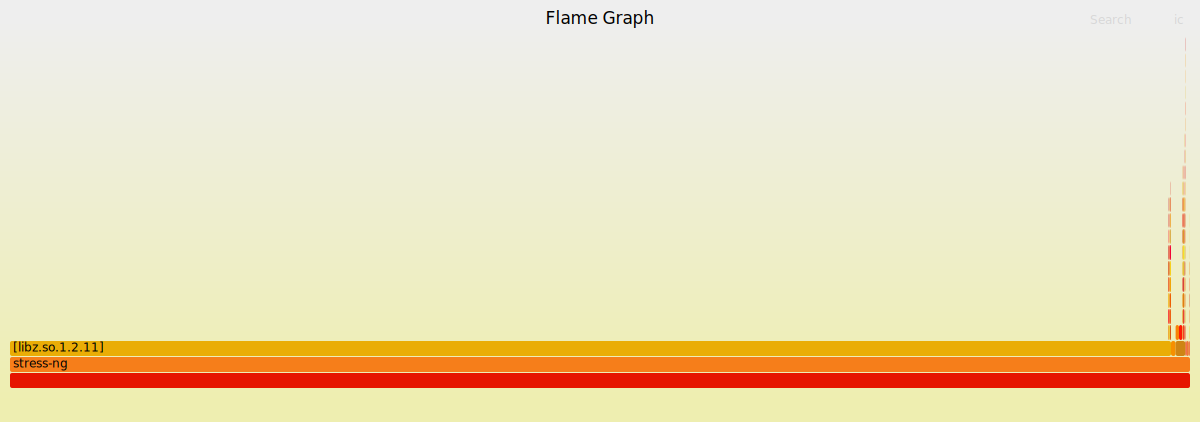
\includegraphics[width=\textwidth]{./memory/image/graph-zlib-test.png}
\subsection{fork-vm}
\nquote{--fork-vm}{enable  detrimental  performance  virtual  memory  advice  using  madvise  on all pages of the forked process. Where possible this will try to set every  page  in  the  new  process  with  using  madvise 
$MADV\_MERGEABLE$, $MADV\_WILLNEED$, $MADV\_HUGEPAGE$ and $MADV\_RANDOM$ flags. Linux only.}
Посмотрим, как изменяется количество свободных страниц виртуальной памяти с помощью \textit{vmstat} при включенной и выключенной опции \textit{fork-vm};\\
\includegraphics[width=\textwidth]{./memory/image/fork-vm.png}
Видим, что особого влияния на количество свободных страниц виртуальной памяти нет.\\
